\documentclass[tikz,border=5pt]{standalone}
\usepackage[T1]{fontenc}
\usepackage{lmodern,amsmath,amssymb}
\usetikzlibrary{arrows.meta,calc,positioning,fit,backgrounds,shapes.geometric,matrix,decorations.pathreplacing,patterns}
\definecolor{ink}{gray}{0.08}
\definecolor{wash}{gray}{0.965}
\definecolor{soft}{gray}{0.45}
\tikzset{box/.style={draw=ink,line width=.65pt,fill=white,align=center,inner sep=4pt,outer sep=0pt,font=\small},flow/.style={draw=ink,line width=.65pt,-{Latex[length=1.8mm,width=1.3mm]},rounded corners=2pt},annotation/.style={font=\scriptsize,text=soft,align=center},groupbox/.style={draw=soft,dashed,line width=.45pt,fill=wash}}
\begin{document}
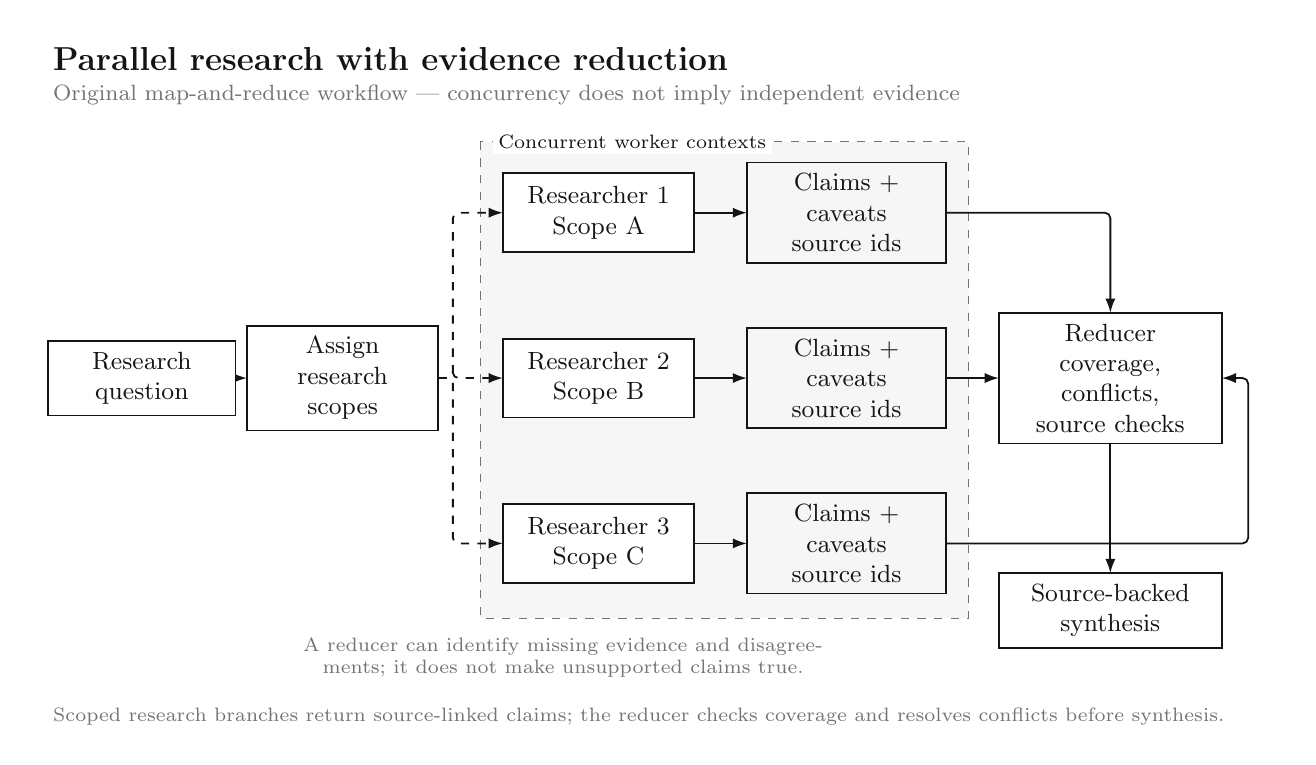
\begin{tikzpicture}[x=1cm,y=-1cm,font=\rmfamily,text=ink]

\path[use as bounding box] (0,0) rectangle (16,9);
\node[anchor=west,font=\large\bfseries] at (.2,.4) {Parallel research with evidence reduction};
\node[anchor=west,font=\footnotesize,text=soft] at (.2,.85) {Original map-and-reduce workflow | concurrency does not imply independent evidence};
\begin{pgfonlayer}{background}
\draw[groupbox] (5.75,1.45) rectangle (11.95,7.5);
\node[anchor=west,font=\scriptsize,fill=white,inner sep=2pt] at (5.9,1.45) {Concurrent worker contexts};
\end{pgfonlayer}
\node[box,minimum width=2.35cm,minimum height=0.95cm,text width=2.1cm] (question) at (1.45,4.45) {Research question};
\node[box,minimum width=2.4cm,minimum height=1.1cm,text width=2.15cm] (scope) at (4.0,4.45) {Assign\\research scopes};
\node[box,minimum width=2.4cm,minimum height=1.0cm,text width=2.15cm] (worker1) at (7.25,2.35) {Researcher 1\\Scope A};
\node[box,fill=wash,minimum width=2.5cm,minimum height=1.15cm,text width=2.25cm] (evidence1) at (10.4,2.35) {Claims + caveats\\source ids};
\node[box,minimum width=2.4cm,minimum height=1.0cm,text width=2.15cm] (worker2) at (7.25,4.45) {Researcher 2\\Scope B};
\node[box,fill=wash,minimum width=2.5cm,minimum height=1.15cm,text width=2.25cm] (evidence2) at (10.4,4.45) {Claims + caveats\\source ids};
\node[box,minimum width=2.4cm,minimum height=1.0cm,text width=2.15cm] (worker3) at (7.25,6.55) {Researcher 3\\Scope C};
\node[box,fill=wash,minimum width=2.5cm,minimum height=1.15cm,text width=2.25cm] (evidence3) at (10.4,6.55) {Claims + caveats\\source ids};
\node[box,minimum width=2.8cm,minimum height=1.35cm,text width=2.55cm] (reduce) at (13.75,4.45) {Reducer\\coverage, conflicts,\\source checks};
\node[box,minimum width=2.8cm,minimum height=0.9cm,text width=2.55cm] (synthesis) at (13.75,7.4) {Source-backed\\synthesis};
\begin{pgfonlayer}{background}
\draw[flow,dashed] (scope.east) -- (5.4,4.45) -- (5.4,2.35) -- (worker1.west);
\draw[flow] (worker1.east) -- (evidence1.west);
\draw[flow,dashed] (scope.east) -- (5.4,4.45) -- (5.4,4.45) -- (worker2.west);
\draw[flow] (worker2.east) -- (evidence2.west);
\draw[flow,dashed] (scope.east) -- (5.4,4.45) -- (5.4,6.55) -- (worker3.west);
\draw[flow] (worker3.east) -- (evidence3.west);
\draw[flow] (question.east) -- (scope.west);
\draw[flow] (evidence1.east) -- (13.75,2.35) -- (reduce.north);
\draw[flow] (evidence2.east) -- (reduce.west);
\draw[flow] (evidence3.east) -- (15.5,6.55) -- (15.5,4.45) -- (reduce.east);
\draw[flow] (reduce.south) -- (synthesis.north);
\end{pgfonlayer}
\node[annotation,anchor=center,text width=10.7cm] at (6.8,8.0) {A reducer can identify missing evidence and disagreements; it does not make unsupported claims true.};
\node[anchor=west,align=left,font=\scriptsize,text=soft,text width=15.6cm] at (.2,8.75) {Scoped research branches return source-linked claims; the reducer checks coverage and resolves conflicts before synthesis.};
\end{tikzpicture}
\end{document}
